\documentclass[CJKutf8,xcolor=pdftex,dvipsnames,table]{beamer}
\usepackage{hyperref}
\hypersetup{
  pdftitle={Operating System Concepts},
  pdfauthor={Hong MingJian},
  pdfsubject={Operating system structures},
  pdfpagemode={FullScreen},
  colorlinks={true},
  linkcolor={blue},
}
\usepackage{CJKutf8}

\usetheme{Madrid}%{Warsaw}
\usecolortheme{crane}

\begin{document}
\begin{CJK*}{UTF8}{song}

  \title{\CJKfamily{hei} 操作系统原理}
  \subtitle{\CJKfamily{hei} 第三章:操作系统结构}
  \author{\CJKfamily{hei} 洪明坚}
  \institute{\CJKfamily{hei} 重庆大学软件学院}
  \date{\today}

  \AtBeginSection[]
  {
    \begin{frame}
      \frametitle{Outline}
      \tableofcontents[currentsection]
    \end{frame}
  }

  \frame{\titlepage}

  \frame{\frametitle{目录}\tableofcontents}

  \section{Operating system structures}

  \iffalse

  %% PAGE
  \begin{frame}
    \frametitle{Operating system structures} \pause
    \begin{itemize}
    \item{An operating system may be viewed from several vantage points:} \pause
      \begin{itemize}
      \item{\textbf{Component view} \pause - What does an operating system consist of?} \pause
      \item{\textbf{Service view} \pause - What the operating system can do for \textbf{users}?} \pause
      \item{\textbf{Interface view} \pause - How do the \textbf{programmers} interact with the operating system?} \pause
      \item{\textbf{Structure view} \pause - How did the \textbf{system designers} design the operating system?}
      \end{itemize}
    \end{itemize}
  \end{frame}

  \subsection{Component view}

  %% PAGE
  \begin{frame}
    \frametitle{Component view} \pause
    \begin{itemize}
    \item{Most modern operating systems consist of the following components:} \pause
      \begin{itemize}
      \item{\textbf{CPU management}} \pause
      \item{\textbf{Memory management}} \pause
      \item{\textbf{File management}} \pause
      \item{I/O management} \pause
      \item{Networking}  \pause
      \item{Protection} \pause
      \item{Command-interpreter system (or \textbf{shell}), which is the interface between the user and the operating system. Two flavors:} \pause
        \begin{itemize}
        \item{\textbf{Command-line interpreter} in text mode \pause - gets the next command and executes it.} \pause
        \item{\textbf{Graphical User Interface (GUI)} in graphical mode \pause - user-friendly mouse-based window-and-menu system.}
        \end{itemize}
      \end{itemize}
    \end{itemize}
  \end{frame}

  \subsection{Service view}

  %% PAGE
  \begin{frame}
    \frametitle{Service view (1/2)} \pause
    \begin{itemize}
    \item{The operating system provides certain services to programs and users:} \pause
      \begin{itemize}
      \item{Program execution \pause - Load a program into memory and run it.} \pause
      \item{I/O operations} \pause
      \item{File-system manipulation} \pause
      \item{Error detection} \pause
      \item{Communications \pause - Exchange information between two or more processes.}\\ \pause
        \begin{minipage}[c]{0.4\textwidth}
          \begin{itemize}
          \item{\textbf{Shared memory} for processes executing on the same computer;} \pause
          \item{\textbf{Message passing} for processes executing on the same or different computers.} \pause
          \end{itemize}
        \end{minipage}%
        \begin{minipage}[c]{0.6\textwidth}
          % \begin{center}
          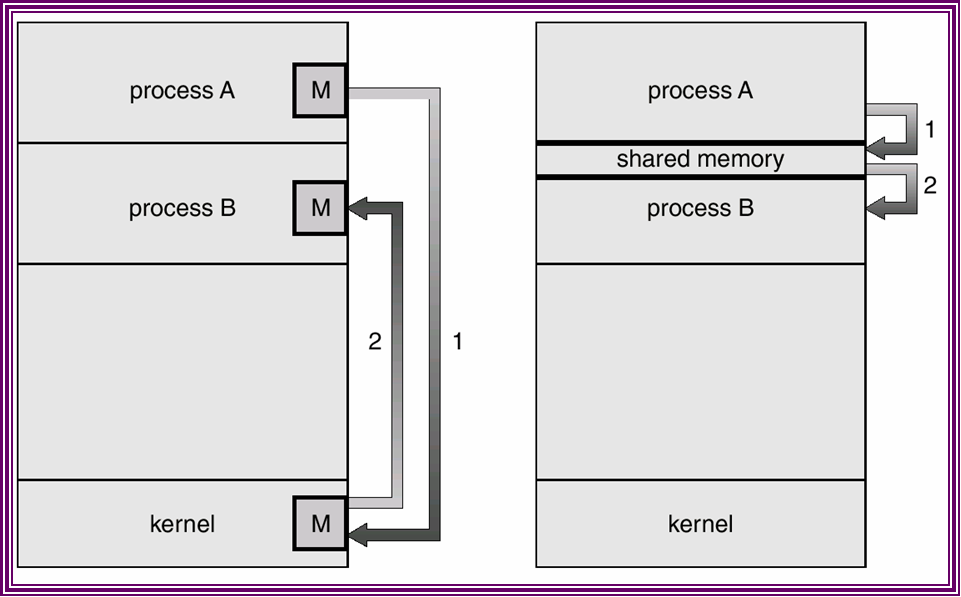
\includegraphics[scale=0.35]{v6f3-5}
          % \end{center}
        \end{minipage}
      \end{itemize}
    \end{itemize}
  \end{frame}

  %% PAGE
  \begin{frame}
    \frametitle{Service view (2/2)} \pause
    \begin{itemize}
    \item{Additional functions exist not for helping the user, but rather for ensuring efficient system operations.} \pause
      \begin{itemize}
      \item{Resource allocation} \pause
      \item{Accounting} \pause
      \item{Protection}
      \end{itemize}
    \end{itemize}
  \end{frame}

  \subsection{Interface view}

  %% PAGE
  \begin{frame}
    \frametitle{Interface view - System calls (1/2)} \pause
    \begin{itemize}
    \item{System calls provide the interface between a running program and the operating system.} \pause
      \begin{itemize}
      \item{Generally available as assembly-language instructions.} \pause
      \item{Other languages must wrap the assembly-language instructions to access services provided by the operating system.} \pause
      \end{itemize}
    \item{Three general methods are used to pass parameters between a running program and the operating system.} \pause
      \begin{itemize}
      \item{Pass parameters in registers.} \pause
      \item{Store the parameters in a table in memory, and the table address is passed as a parameter in a register.} \pause
      \item{Push the parameters onto the stack by the program, and pop off the stack by operating system.}
      \end{itemize}
    \end{itemize}
  \end{frame}

  %% PAGE
  \begin{frame}
    \frametitle{Interface view - System calls (2/2)} \pause
    \begin{itemize}
    \item{Process control} \pause
      \begin{itemize}
      \item{Create process such as \textbf{fork} in Unix/Linux and \textbf{spawn} in MS-DOS.} \pause
      \item{Wait event and signal event.} \pause
      \item{Allocate and free memory.} \pause
      \end{itemize}
    \item{File management} \pause
      \begin{itemize}
      \item{Create, open, read/write, close and delete file} \pause
      \end{itemize}
    \item{Device management} \pause
      \begin{itemize}
      \item{Logically attach/detach, read, write device} \pause
      \end{itemize}
    \item{Information maintenance} \pause
      \begin{itemize}
      \item{get/set time or date} \pause
      \end{itemize}
    \item{Communications} \pause
      \begin{itemize}
      \item{create/delete communication connection, send/receive message}
      \end{itemize}
    \end{itemize}
  \end{frame}

  %% PAGE
  \begin{frame}
    \frametitle{Interface view - system programs} \pause
    \begin{itemize}
    \item{System programs provide a convenient environment for program development and execution. They can be divided into:} \pause
      \begin{itemize}
      \item{The shell} \pause
      \item{File management} \pause
      \item{Status information} \pause
      \item{File modification} \pause
      \item{Programming-language support} \pause
      \item{Program loading an execution} \pause
      \item{Communications} \pause
      \end{itemize}
    \item{Most users' view of the operation system is defined by system programs, not the actual system calls.}
    \end{itemize}
  \end{frame}

  %% PAGE
  \begin{frame}
    \frametitle{Questions}
    \begin{itemize}
    \item{Any questions?}
    \end{itemize}
    \begin{center}
      
\includegraphics[scale=.5]{question}
    \end{center}
  \end{frame}

  \section{System structure}
  \fi


  %% PAGE
  \begin{frame}
    \frametitle{System structure} \pause
    \begin{itemize}
    \item{A system as large and complex as a modern operating system must be engineered carefully if it's to function properly and be modified easily.} \pause
    \item{A common approach is to partition the task into small components, rather than have one monolithic system.} \pause
      \begin{itemize}
      \item{Each of these components should be a well-defined portion of the system, with carefully defined inputs, outputs and function.} \pause
      \end{itemize}
    \item{How does the system designer organize these components?} \pause
      \begin{itemize}
      \item{Simple structure (or no structure)} \pause
      \item{Layered structure} \pause
      \item{Micro-kernel} \pause
      \item{Virtual machine}
      \end{itemize}
    \end{itemize}
  \end{frame}

  \subsection{Simple structure}

  %% PAGE
  \begin{frame}
    \frametitle{Simple structure} \pause
    \begin{itemize}
    \item{Many systems do not have a well-defined structure.} \pause
      \begin{itemize}
      \item{They started as small, simple and limited system, and then evolved into a complex one.} \pause
      \end{itemize}
    \item{Examples: MS-DOS and Unix} \pause
    \end{itemize}
    \begin{minipage}[c]{0.5\textwidth}
      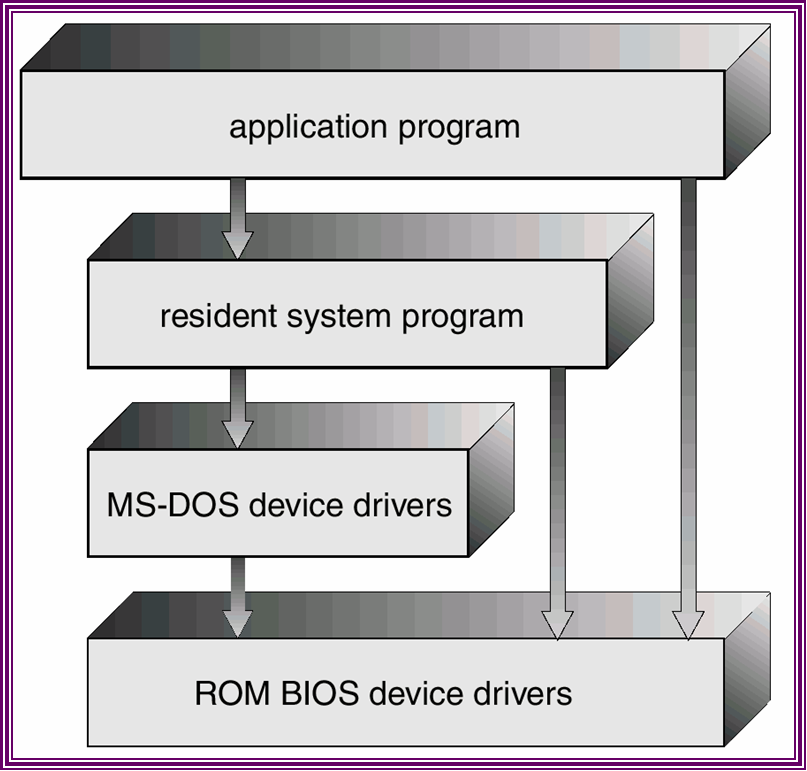
\includegraphics[scale=0.4]{v6f3-6} \pause
    \end{minipage}%
    \begin{minipage}[c]{0.5\textwidth}
      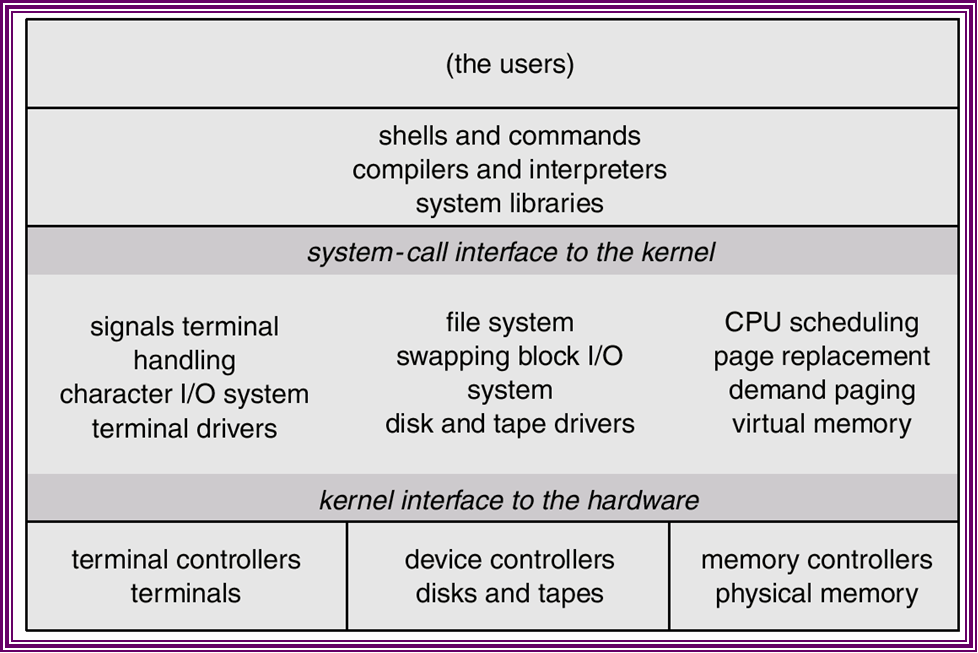
\includegraphics[scale=0.35]{v6f3-7}
    \end{minipage}
  \end{frame}

  \subsection{Layered structure}

  %% PAGE
  \begin{frame}
    \frametitle{Layered structure (1/4)} \pause
    \begin{itemize}
    \item{The operating system is broken up into a number of layers, each built on top lower layers.} \pause
    \end{itemize}
    \begin{center}
      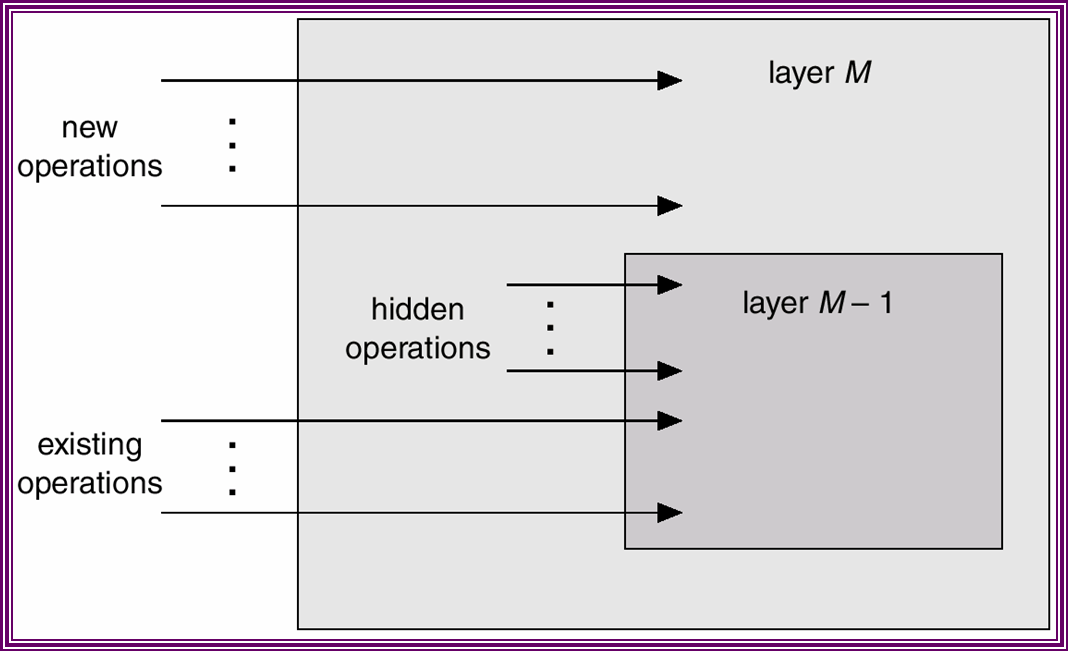
\includegraphics[scale=0.5]{v6f3-8}
    \end{center}
  \end{frame}

  %% PAGE
  \begin{frame}
    \frametitle{Layered structure (2/4)} \pause
    \begin{itemize}
    \item{Example 1:} \pause
      \begin{itemize}
      \item{The \textbf{THE} operating system by Dijkstra.}
      \end{itemize}
    \end{itemize}
    \begin{center}
      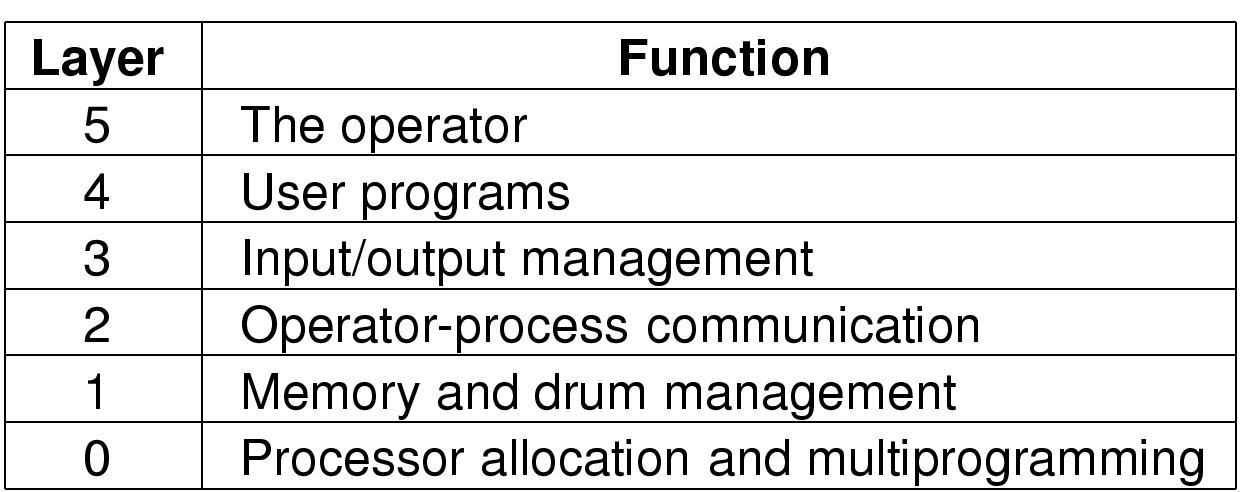
\includegraphics[scale=.2]{mosv2f1-25}
    \end{center}
  \end{frame}

  %% PAGE
  \begin{frame}
    \frametitle{Layered structure (3/4)} \pause
    \begin{itemize}
    \item{Example 2:} \pause
      \begin{itemize}
      \item{The IBM OS/2 operating system} \pause
      \end{itemize}
    \end{itemize}
    \begin{center}
      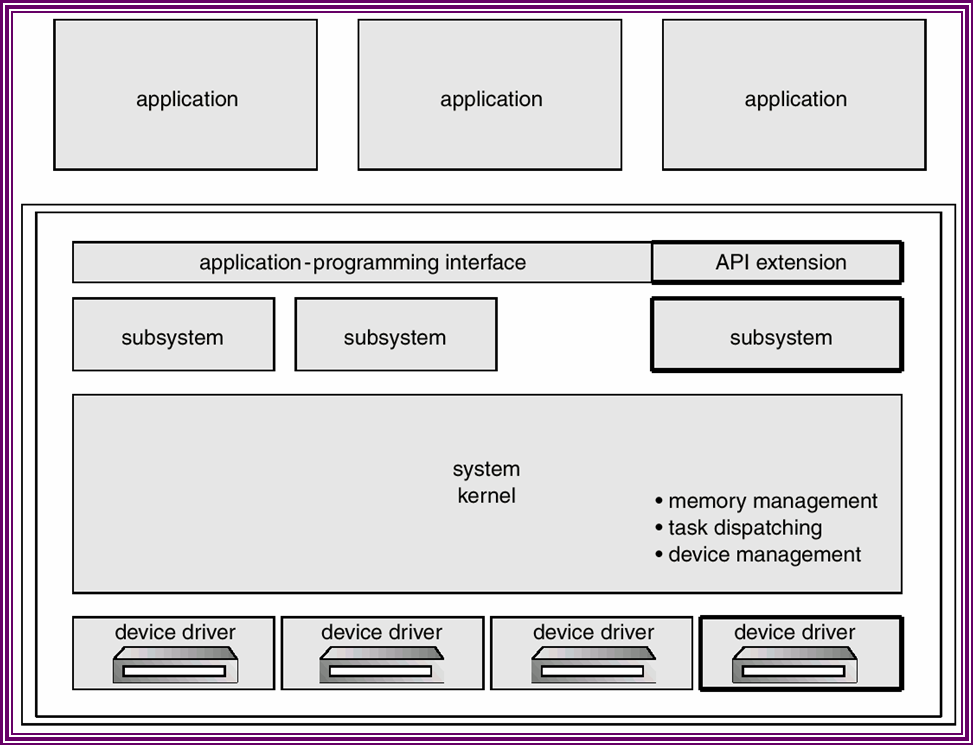
\includegraphics[scale=0.5]{v6f3-9}
    \end{center}
  \end{frame}
  
  %% PAGE
  \begin{frame}
    \frametitle{Layered structure (4/4)} \pause
    \begin{itemize}
    \item{The major difficulty with the layered structure involves} \pause
      \begin{enumerate}
      \item{careful definition of the layers and} \pause
      \item{less efficient.}
      \end{enumerate}
    \end{itemize}
  \end{frame}
  
  \subsection{Micro-kernel}

  %% PAGE
  \begin{frame}
    \frametitle{Micro-kernel (1/2)} \pause
    \begin{itemize}
    \item{As the Unix operating system expanded, the kernel became large and difficult to manage.} \pause
      \begin{itemize}
      \item{The \textbf{micro-kernel} approach structures the operating system by removing all non-essential components from the kernel and implementing them as system- and user-level programs.} \pause
      \end{itemize}
    \item{Which components should remain in the micro-kernel?} \pause
      \begin{itemize}
      \item{CPU management} \pause
      \item{Memory management} \pause
      \item{Communication facility} \pause
      \end{itemize}
    \end{itemize}
    \begin{center}
      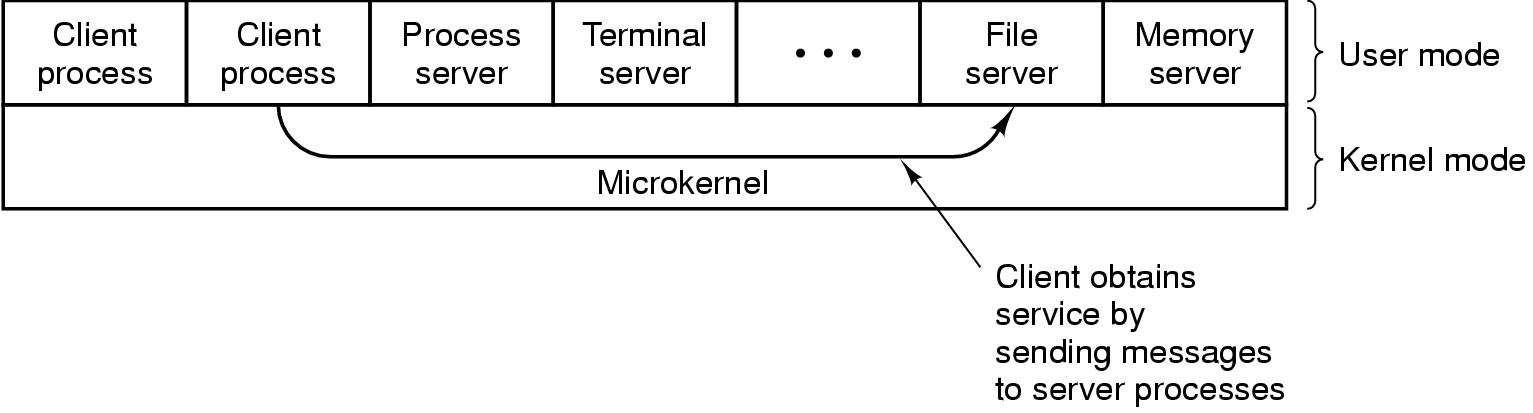
\includegraphics[scale=.2]{mosv2f1-27}
    \end{center}
  \end{frame}
  
  %% PAGE
  \begin{frame}
    \frametitle{Micro-kernel (2/2)} \pause
    \begin{itemize}
    \item{Example 1} \pause
      \begin{itemize}
      \item{The open source \textbf{Mach} from Carnegie Mellon University.} \pause
        \begin{itemize}
        \item{Used as the kernel of the Apple Mac OS X and the DEC Tru64 Unix.} \pause
        \end{itemize}
      \end{itemize}
    \item{Example 2} \pause
      \begin{itemize}
      \item{QNX real-time operating system by QNX Inc.} \pause
      \end{itemize}
    \item{Example 3} \pause
      \begin{itemize}
      \item{Micorsoft Windows NT/XP} \pause
      \end{itemize}
      \begin{center}
        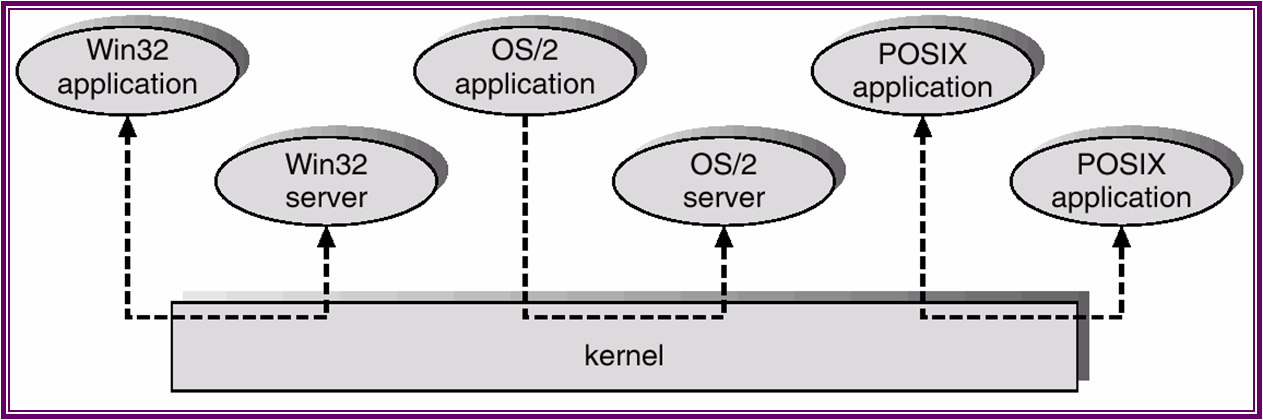
\includegraphics[scale=.45]{v6f3-10}
      \end{center}
    \end{itemize}
  \end{frame}
  
  %% PAGE
  \begin{frame}
    \frametitle{Questions}
    \begin{itemize}
    \item{Any questions?}
    \end{itemize}
    \begin{center}
      
\includegraphics[scale=.5]{question}
    \end{center}
  \end{frame}
  
  \subsection{Virtual machine}

  %% PAGE
  \begin{frame}
    \frametitle{Virtual machine (1/4)} \pause
    \begin{itemize}
    \item{If we take a step further from micro-kernel,} \pause
      \begin{itemize}
      \item{The low-level real hardware is ``cloned'' into several identical \textbf{virtual machines}.} \pause
      \item{That is, virtual machine provides an interface identical to the underlying bare hardware.} \pause
      \end{itemize}
    \item{Then, the operating system functionality is built on top of the virtual machines.}
    \end{itemize}
  \end{frame}
  
  %% PAGE
  \begin{frame}
    \frametitle{Virtual machine (2/4)} \pause
    \begin{itemize}
    \item{Virtual machine structure} \pause
    \end{itemize}
    \begin{center}
      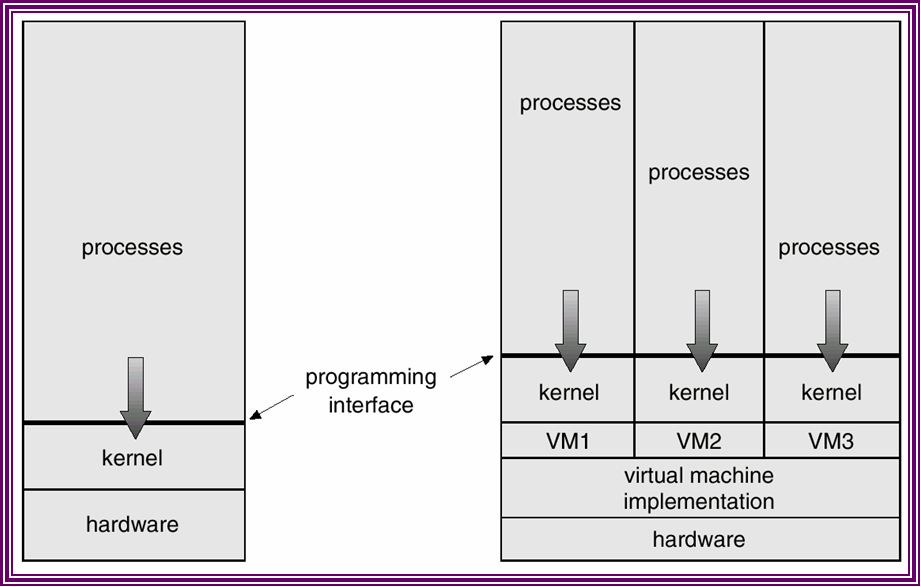
\includegraphics[scale=0.6]{v6f3-11} \pause
    \end{center}
  \end{frame}

  %% PAGE
  \begin{frame}
    \frametitle{Virtual machine (3/4)} \pause
    \begin{itemize}
    \item{Examples} \pause
      \begin{itemize}
      \item{IBM VM/370} \pause
      \item{\htmladdnormallink{Xen}{http://www.xenproject.org/}} \pause
      \item{\htmladdnormallink{KVM (Kernel-based Virtual Machine)}{http://www.linux-kvm.org/page/Main\_Page}} \pause
      \end{itemize}
    \end{itemize}
  \end{frame}
  
  \iffalse

  %% PAGE
  \begin{frame}
    \frametitle{Virtual machine (3/5)} \pause
    \begin{itemize}
    \item{Usually, virtual machines can be classified into two kinds:} \pause
      \begin{itemize}
      \item{\textbf{Hardware virtual machines} \pause - explained above} \pause
      \item{\textbf{Application virtual machines} \pause - a piece of computer software that isolates the application being used by the user from the computer. } \pause
        \begin{itemize}
        \item{Example: Sun microsystem's Java Virtual Machine (JVM).}
        \end{itemize}
      \end{itemize}
    \end{itemize}
  \end{frame}
  

  %% PAGE
  \begin{frame}
    \frametitle{Virtual machine (4/5)} \pause
    \begin{itemize}
    \item{Hardware virtual machines can be implemented in three ways:} \pause
      \begin{itemize}
      \item{\textbf{Emulation} \pause - the virtual machine simulates the complete hardware, allowing an unmodified operating system for a completely different CPU to run.} \pause
        \begin{itemize}
        \item{Examples: VMware, VirtualPC, open-source Bochs, etc.} \pause
        \end{itemize}
      \item{\textbf{Paravirtualization} \pause - the virtual machine does not simulate hardware but instead offers a special API that requires operating system modifications to run.} \pause
        \begin{itemize}
        \item{Examples: Open-source \textbf{Xen} from Cambridge University.} \pause
        \end{itemize}
      \item{\textbf{Native (Full) virtualization} \pause - the virtual machine only partially simulates enough hardware to allow an unmodified operating system to run in isolation, but the \textbf{guest} operating system must be designed for the same type of CPU} \pause
        \begin{itemize}
        \item{Examples: Open-source KVM (Kernel-based Virtual Machine) for Linux and IBM VM/370}
          % \begin{center}
          %   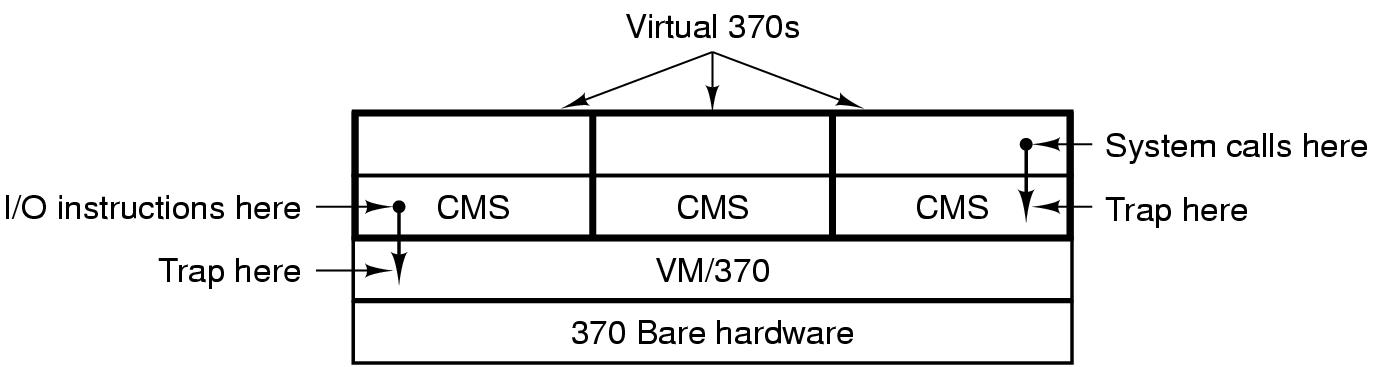
\includegraphics[scale=0.2]{mosv2f1-26} \pause
          % \end{center}
        \end{itemize}
      \end{itemize}
    \end{itemize}
  \end{frame}

  \fi
  
  %% PAGE
  \begin{frame}
    \frametitle{Virtual machine (4/4)} \pause
    \begin{itemize}
    \item{Advantage and disadvantage of virtual machine} \pause
      \begin{itemize}
      \item{The virtual-machine concept provides complete protection of system resources since each virtual machine is isolated from all other virtual machines.} \pause
        \begin{itemize}
        \item{This isolation, however, permits no direct sharing of resources} \pause
        \end{itemize}
      \item{A virtual-machine system is a perfect vehicle for operating-systems research and development.} \pause
      \item{The virtual machine concept is difficult to implement due to the effort required to provide an \textbf{exact} duplicate to the underlying machine.}
      \end{itemize}
    \end{itemize}
  \end{frame}
  
  %% PAGE
  \begin{frame}
    \frametitle{Questions}
    \begin{itemize}
    \item{Any questions?}
    \end{itemize}
    \begin{center}
      
\includegraphics[scale=.5]{question}
    \end{center}
  \end{frame}

  \section{Operating system design}
  
  %% PAGE
  \begin{frame}
    \frametitle{Operating System design} \pause
    \begin{itemize}
    \item{Design goals} \pause
      \begin{description}
      \item[\textbf{User goals}]{operating system should be convenient to use, easy to learn, reliable, safe, and fast.} \pause
      \item[\textbf{System goals}]{operating system should be easy to design, implement, and maintain, as well as flexible, reliable, error-free, and efficient.}
      \end{description}
    \end{itemize}
  \end{frame}
  
  \subsection{Policy and mechanism}

  %% PAGE
  \begin{frame}
    \frametitle{Policy and mechanism} \pause
    \begin{itemize}
    \item{\textbf{Policies \pause - what to do}} \pause
      \begin{itemize}
      \item{For example, users should not be able to read other users' files.} \pause
      \end{itemize}
    \item{\textbf{Mechanisms \pause - how to do}} \pause
      \begin{itemize}
      \item{For example, file permissions are checked on \emph{open} system call.} \pause
      \end{itemize}
    \item{The \textbf{separation} of policy from mechanism is a very important principle} \pause
      \begin{itemize}
      \item{It allows maximum flexibility if policy decisions are to be changed later.} \pause
      \end{itemize}
    \item{Two extremes:} \pause
      \begin{itemize}
      \item{Micro-kernel \pause - all mechanisms, almost no policy} \pause
      \item{The Apple Macintosh \pause - policy and mechanism are bound together}
      \end{itemize}
    \end{itemize}
  \end{frame}

  \subsection{Implementation}
  
  %% PAGE
  \begin{frame}
    \frametitle{The operating system implementation} \pause
    \begin{itemize}
    \item{Traditionally written in assembly language, operating systems can now be written in higher-level languages.} \pause
    \item{Code written in a high-level language:} \pause
      \begin{itemize}
      \item{can be written faster.} \pause
      \item{is more compact.} \pause
      \item{is easier to understand and debug.} \pause
      \item{is easier to port to some other hardwares.}
      \end{itemize}
    \end{itemize}
  \end{frame}
  
  %% PAGE
  \begin{frame}
    \frametitle{Questions}
    \begin{itemize}
    \item{Any questions?}
    \end{itemize}
    \begin{center}
      
\includegraphics[scale=.5]{question}
    \end{center}
  \end{frame}
  
  %% PAGE
\end{CJK*}
\end{document}
